\documentclass[11pt]{book}
\usepackage[slovene]{babel}
\usepackage[utf8]{inputenc}
\usepackage{amsmath}
\usepackage[dvipsnames]{xcolor}
\usepackage{titlesec}
% \usepackage{amssymb}
\usepackage{pstricks,pst-plot,pst-math}
\usepackage{pstricks-add}
\usepackage{graphicx}
\usepackage{enumerate}
\usepackage{color}
\usepackage{fouriernc}
\usepackage{microtype}
\usepackage{MnSymbol}
\usepackage{tikz-cd}
\usetikzlibrary{backgrounds}
\usepackage{wrapfig}
\usepackage{geometry}
\geometry{
    a4paper,
    left=45mm,
    right=45mm,
    top=20mm,
    bottom=20mm
    }
    \usepackage{comment}
    

\usepackage{amsthm}

\usepackage{changepage}   % for the adjustwidth environment
\usepackage{hyperref}
\hypersetup{
    colorlinks=true,
    linkcolor=cyan,
    filecolor=magenta,      
    urlcolor=cyan
    }

\usepackage[backgroundcolor=svetlosiva,linecolor=siva,textsize=footnotesize]{todonotes}

\pagestyle{plain}

\usepackage{enumitem}
\setlist[description]{leftmargin=\parindent,labelindent=\parindent, font=\normalfont\itshape\textbullet\space}


\def\NN{\mathbf{N}}
\def\ZZ{\mathbf{Z}}
\def\QQ{\mathbf{Q}}
\def\RR{\mathbf{R}}
\def\CC{\mathbf{C}}
\def\conclass{\mathcal{C}}
\def\11{\mathbf{1}}
\def\FF{\mathbf{F}}
\def\Fcal{\mathcal{F}}
\def\EE{\mathbf{E}}
\def\PP{\mathbf{P}}
\def\HH{\mathbf{H}}
\def\youngsym{\sigma_{\lambda}}

\DeclareMathOperator\image{im}
\DeclareMathOperator\sgn{sgn}
\DeclareMathOperator\Res{Res}
\DeclareMathOperator\Ind{Ind}
\DeclareMathOperator\Rep{Rep}
\DeclareMathOperator\mult{mult}
\DeclareMathOperator\Izotip{Izotip}
\DeclareMathOperator\MK{MK}
\DeclareMathOperator\tr{tr}
\DeclareMathOperator\Irr{Irr}
\DeclareMathOperator\SU{SU}
\DeclareMathOperator\characteristic{char}
\DeclareMathOperator\kk{k}
\DeclareMathOperator\cl{cl}
\def\GAP{\texttt{GAP}}
\DeclareMathOperator\inv{inv}
\DeclareMathOperator\Eigenvalues{Spec}
\DeclareMathOperator\Eigenspace{ES}
\DeclareMathOperator\fun{fun}
\DeclareMathOperator\HS{HS}
\DeclareMathOperator\St{St}
\DeclareMathOperator\Realpart{Re}

\DeclareMathOperator\DNO{DNO}
\DeclareMathOperator\KNO{KNO}


\DeclareMathOperator\Aut{Aut}
\DeclareMathOperator\GL{GL}
\DeclareMathOperator\glfrak{\mathfrak{gl}}
\DeclareMathOperator\slfrak{\mathfrak{sl}}
\DeclareMathOperator\U{U}
\DeclareMathOperator\SL{SL}
\DeclareMathOperator\PSL{PSL}
\DeclareMathOperator\SO{SO}
\DeclareMathOperator\Gal{Gal}
\DeclareMathOperator\Sym{Sym}
\DeclareMathOperator\Homeo{Homeo}
\DeclareMathOperator\Cay{Cay}
\DeclareMathOperator\Isom{Isom}
\DeclareMathOperator\id{id}
\DeclareMathOperator\supp{supp}
\DeclareMathOperator\End{End}
\DeclareMathOperator\Mat{Mat}
\DeclareMathOperator\Cone{Cone}
\DeclareMathOperator\diam{diam}
\DeclareMathOperator\Ad{Ad}
\DeclareMathOperator\imaginary{Im}

\def\definicija{\color{rdeca}\bf\em}
\def\vprasanje{\color{oranzna}}
\def\literatura{\color{modra}}
\def\vaje{{\literatura ($\to$ vaje)}}
\def\kljuka{$\checkmark$}

\theoremstyle{definition}

\newtheoremstyle{zgled}
 {}{}%
 {\color{zelena}}
 {}%
 {\color{zelena}\bfseries}%
 {\color{zelena}.}%
 { }{}

\theoremstyle{zgled}
\newtheorem*{zgled}{Zgled}

\newtheoremstyle{odprtproblem}
 {}{}%
 {\color{oranzna}}
 {}%
 {\color{oranzna}\bfseries}%
 {\color{oranzna}.}%
 { }{}

\theoremstyle{odprtproblem}
\newtheorem*{odprtproblem}{Odprt problem}

\newtheoremstyle{domacanaloga}
 {}{}%
 {\color{vijolicna}}
 {}%
 {\color{vijolicna}\bfseries}%
 {\color{vijolicna}.}%
 { }{}

\theoremstyle{domacanaloga}
\newtheorem*{domacanaloga}{Domača naloga}

\newenvironment{dokaz}
    {\color{siva}\begin{proof}}
    {\end{proof}}

\newtheoremstyle{izrek}
 {}{}% above, below 
 {\color{black}\itshape}
 {}% indent
 {\color{black}\bfseries}%
 {\color{black}.}%
 { }{}

\theoremstyle{izrek}
\newtheorem*{izrek}{Izrek}

\newtheorem*{trditev}{Trditev}
\newtheorem*{pomoznatrditev}{Pomožna trditev}

\newtheorem*{lema}{Lema}

\newtheorem*{posledica}{Posledica}

\newenvironment{povzetek}
    {
\smallskip
\begin{center}
\color{svetlosiva}
\begin{tabular}{|p{0.7\textwidth}}
    }
    {
\end{tabular}
\end{center}
\smallskip
    }


\definecolor{rdeca}{rgb}{0.62, 0.16, 0.10}
\definecolor{zelena}{rgb}{0.15, 0.4, 0.20}
\definecolor{oranzna}{rgb}{0.72, 0.38, 0.082}
\definecolor{rjava}{rgb}{0.7490196078431373, 0.3686274509803922, 0.1843137254901961}
\definecolor{modra}{rgb}{0.2784313725490196, 0.5411764705882353, 0.8392156862745098}
\definecolor{vijolicna}{rgb}{0.48627450980392156, 0.2980392156862745, 0.792156862745098}
\definecolor{siva}{rgb}{0.5, 0.5, 0.5}
\definecolor{svetlosiva}{rgb}{0.7, 0.7, 0.7}


\titleformat{\section}
  {\color{rdeca}\LARGE\bf}{\thesection}{1em}{}
\renewcommand{\thesubsection}{}
\titleformat{\subsection}
  {\Large\bf}{}{1em}{}

\title{\bf Diskretne stukture}
\author{Urban Jezernik}

% za generiranje html dokumenta s stilom mystyle.css uporabi:
% pandoc ds.tex --toc --toc-depth=2 --metadata date="`date -u "+%d. %m. %Y"`" --template template.html -c mystyle.css -s --mathjax -o index.html


\begin{document}

\baselineskip=14pt

\maketitle

\setcounter{tocdepth}{1}
\tableofcontents

\newpage

\subsection*{Kratek opis predmeta}

Pri predmetu se bomo najprej naučili, kaj točno so \emph{izjave} in kako jih matematično \emph{formalizirati}. Eden pomembnih ciljev tega je eksakten opis  \emph{sklepanja}, ki ga uporabljamo počez matematike. Te koncepte bomo najprej razvili v osnovnem \emph{izjavnem računu}, nato pa ga bomo še posplošili do \emph{predikatnega računa}, s katerim bomo podrobneje raziskali matematične izjave. 

\begin{zgled}
Nepridipravi so razbili vhodna vrata FMF. Glavni osumljenci so študenti Ana, Bor in Cveto. Ko jih vprašamo, kdo je kriv, odgovorijo z naslednjimi izjavami:

\begin{itemize}
    \item Ana: ``Bor je kriv, Cveto pa ne.''
    \item Bor: ``Če je kriva Ana, je kriv tudi Cveto.''
    \item Cveto: ``Jaz nisem kriv, toda vsaj eden od drugih dveh je kriv.''
\end{itemize}

Pri predmetu se bomo naučili, kako lahko na \emph{sistematičen način} odkrijemo, kdo je lagal, če krivi lažejo, nedolžni pa govorijo resnico.
\end{zgled}

Za tem bomo pri predmetu spoznali nekaj osnovnih diskretnih struktur, po katerih se ta predmet imenuje. Najprej bomo raziskali \emph{relacije}, s katerimi opisujemo odnose med elementi dane množice. Pomemben poseben primer teh so \emph{urejenosti}, ki posplošujejo običajne ureditve števil po velikosti. Najbolj podrobno si bomo ogledali \emph{grafe}, s katerimi lahko abstraktno predstavimo mnogo pomembnih primerov relacij.

\begin{zgled}
Graf je diskretna struktura, pri kateri dano množico \emph{vozlišč} povežemo s \emph{povezavami}. Z grafi lahko opišemo veliko različnih vrst omrežij, na primer internetno omrežje, omrežje prijateljskih povezav na Facebooku, omrežja veriženja blokov (kriptovalute) \dots 

Konkreten graf na spodnji sliki se imenuje {\definicija Petersenov graf}. Ta graf bomo tekom predmeta večkrat srečali. Na koncu predmeta bomo znali \emph{dokazati}, da se tega grafa ne da narisati v ravnini, brez da bi se vsaj dve povezavi sekali.

\begin{figure}[h]
    \centering
    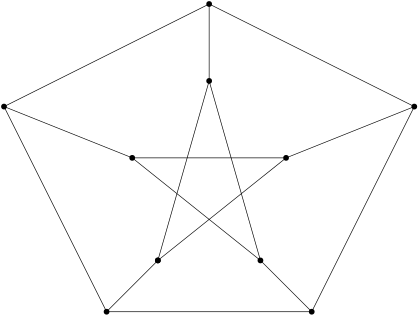
\includegraphics[width=0.5\linewidth]{img/opis-petersen.png}
    \caption{Petersenov graf}
\end{figure}
\end{zgled}

\newpage

\subsection*{Literatura}

\begin{itemize}
\item {\literatura G. Fijavž, \href{http://matematika.fri.uni-lj.si/ds/ds.pdf}{\emph{Diskretne strukture}}, elektronska knjiga, 2015.} 
\item {\literatura M. Juvan in P. Potočnik, \emph{Teorija grafov in kombinatorika}, DMFA-založništvo, Ljubljana 2000.}
\item {\literatura N. Prijatelj, \emph{Osnove matematične logike I}, DMFA-založništvo, Ljubljana, 1992.}
\end{itemize}

\todo{Dodaj literaturo za vaje.}

\chapter{Izjavni račun}

V tem poglavju si bomo pogledali, kako \emph{formaliziramo} preproste izjave in kako \emph{dokazujemo} njihovo veljavnost oziroma neveljavnost.

\section{Izjave in izjavni vezniki}

{\definicija Izjava} je poved, ki je bodisi resnična bodisi lažna.

\begin{zgled} \leavevmode
\begin{itemize}
    \item Ena in ena je tri. \emph{Lažna izjava.}
    \item Ena in ena je dve. \emph{Resnična izjava.}
    \item Koliko je ena in ena? \emph{Ni izjava.}
    \item Pojdimo na kavo! \emph{Ni izjava.}
\end{itemize}
\end{zgled}

Izjave lahko razdelimo na dve skupini \emph{po vsebini}, in sicer:
\begin{itemize}
    \item {\definicija resnične izjave}, ki imajo resničnostno vrednost $1$ ali $\top$ ali \texttt{true},
    \item {\definicija lažne izjave}, ki imajo resničnostno vrednost $0$ ali $\bot$ ali \texttt{false}.
\end{itemize}
Po \emph{zgradbi} oziroma \emph{obliki} pa izjave razdelimo na:
\begin{itemize}
    \item {\definicija osnovne}, ki ne vsebujejo izjavnih veznikov,
    \item {\definicija sestavljene}, ki vsebujejo izjavne veznike.
\end{itemize}

\begin{zgled} \leavevmode
\begin{itemize}
    \item Vreme je lepo. \emph{Osnovna izjava.}
    \item Špela gre v hribe. \emph{Osnovna izjava.}
    \item Vreme je lepo \emph{in} Špela gre v hribe. \emph{Sestavljena izjava.}
    \item \emph{Če} je vreme lepo, \emph{potem} gre Špela v hribe. \emph{Sestavljena izjava.}
    \item Špela \emph{ne} gre v hribe. \emph{Sestavljena izjava.}
\end{itemize}
\end{zgled}

Naj bo $n \in \NN_0$. {\definicija Izjavni veznik reda $n$} (ali {\definicija $n$-mestni izjavni veznik}) je funkcija, ki vsaki urejeni $n$-terici ničel in enic priredi vrednost $0$ ali $1$.

\begin{zgled} \leavevmode
\begin{itemize}
    \item Primer izjavnega veznika reda $1$ je {\definicija negacija}. Simbol za ta veznik je $\lnot$. Če je $p$ izjava, njeno negacijo označimo kot $\lnot p$ in preberemo kot \emph{ne $p$} ali kot \emph{ni res, da velja $p$}. Negacija $1$-terici $0$ priredi vrednost $1$, $1$-terici $1$ pa priredi vrednost $0$.
    
    \begin{table}[h]
        \centering
        \begin{tabular}{c|c}
            $p$ & $\lnot p$ \\ \hline
            0 & 1 \\
            1 & 0
        \end{tabular}
        \caption{Resničnostna tabela negacije}
    \end{table}

    \item Oglejmo si nekaj pomembnih dvomestnih izjavnih veznikov. Njihovi predpisi so zbrani v tabeli.
    \begin{itemize}
        \item {\definicija Konjunkcija} izjav $p$ in $q$ ima simbol $p \land q$, kar preberemo kot \emph{$p$ in $q$}.
        \item {\definicija Disjunkcija} izjav $p$ in $q$ ima simbol $p \lor q$, kar preberemo kot \emph{$p$ ali $q$}.
        \item {\definicija Implikacija} izjav $p$ in $q$ ima simbol $p \Rightarrow q$, kar preberemo kot \emph{če $p$, potem $q$} ali kot \emph{iz $p$ sledi $q$} ali kot \emph{$p$ je zadosten pogoj za $q$} ali \emph{kot $q$ je potreben pogoj za $p$}.
        \item {\definicija Ekvivalenca} izjav $p$ in $q$ ima simbol $p \Leftrightarrow q$, kar preberemo kot \emph{$p$ natanko tedaj, ko $q$} ali kot \emph{$p$, če in samo če $q$} ali kot \emph{$p$ je ekvivalentno $q$}.
    \end{itemize}

    \begin{table}[h]
        \centering
        \begin{tabular}{cc|cccc}
            $p$ & $q$ & $p \land q$ & $p \lor q$ & $p \Rightarrow q$ & $p \Leftrightarrow q$ \\ \hline
            1 & 1 & 1 & 1 & 1 & 1 \\
            1 & 0 & 0 & 1 & 0 & 0 \\
            0 & 1 & 0 & 1 & 1 & 0 \\
            0 & 0 & 0 & 0 & 1 & 1
        \end{tabular}
        \caption{Resničnostna tabela nekaterih pomembnih dvomestnih izjavnih veznikov}
    \end{table}

    \item Izjavni veznik reda $0$ je funkcija iz množice urejenih $0$-teric ničel in enic. Obstaja natanko ena taka $0$-terica, in sicer \emph{prazna $0$-terica}. Izjavni veznik reda $0$ je torej natanko določen s sliko te $0$-terice, za kar imamo dve možnosti, $0$ ali $1$.
    \begin{itemize}
        \item Izjavni veznik reda $0$, ki ima vselej resničnostno vrednost $0$, imenujemo {\definicija 0} in preberemo kot \emph{lažna izjava}.
        \item Izjavni veznik reda $0$, ki ima vselej resničnostno vrednost $1$, imenujemo {\definicija 1} in preberemo kot \emph{resnična izjava}.
    \end{itemize}
    Izjavnima veznikoma reda $0$ pravimo tudi {\definicija izjavni konstanti}.
\end{itemize}
\end{zgled}

Glede na zgornjo obravnavamo izjavnih veznikov redov $0$, $1$ in $2$ se lahko vprašamo, koliko je vseh $n$-mestnih izjavnih veznikov za poljuben $n \in \NN_0$. Vsak tak veznik je enolično določen s svojo resničnostno tabelo, v kateri zabeležimo vrednosti veznika v {\definicija izjavnih spremenljivkah} $p_1, p_2, \dots, p_n$, kjer vsak $p_i$ zavzema vrednosti $0$ ali $1$.

\begin{table}[h]
    \centering
    \begin{tabular}{cccc|c}
        $p_1$ & $p_1$ & $\cdots$ & $p_n$ & veznik($p_1$, $p_2$, \dots, $p_n$) \\ \hline
        1 & 1 & $\cdots$ & 1 & 0 ali 1 \emph{(dve možnosti)} \\
        1 & 1 & $\cdots$ & 0 & 0 ali 1 \emph{(dve možnosti)} \\
        $\vdots$ & $\vdots$ & & $\vdots$ & $\vdots$ \\
        0 & 0 & $\cdots$ & 0 & 0 ali 1 \emph{(dve možnosti)} \\
    \end{tabular}
    \caption{Resničnostna tabela $n$-mestnega izjavnega veznika}
\end{table}

Število vseh $n$-mestnih izjavnih veznikov torej izračunamo tako, da preštejemo število vseh možnih resničnostnih tabel. Število vrstic tabele je enako $2^n$, število vseh tabel pa je zato enako $2^{2^n}$.

\begin{table}[h]
    \centering
    \begin{tabular}{c|cc}
        $n$ & $2^n$ & $2^{2^n}$ \\ \hline
        0 & 1 & 2 \\
        1 & 2 & 4 \\
        2 & 4 & 16 \\
        3 & 8 & 256 \\
        4 & 16 & 65536 \\
        5 & 32 & $\sim 4 \cdot 10^9$ \\
        6 & 64 & $\sim 2 \cdot 10^{19}$
    \end{tabular}
    \caption{Hitra rast števila $n$-mestnih izjavnih veznikov}
\end{table}

\section{Izjavni izrazi}

{\definicija Izjavni izraz} definiramo induktivno na naslednji način:
\begin{itemize}
    \item \emph{Osnovni izraz 1:} Vsaka \emph{izjavna konstanta} (torej $0$ ali $1$) je izjavni izraz. 
    \item \emph{Osnovni izraz 2:} Vsaka \emph{izjavna spremenljivka} $p_1, p_2, \dots$ je izjavni izraz.
    \item \emph{Sestavljeni izraz:} Če je $f$ \emph{izjavni veznik} reda $n$ in so $A_1, A_2, \dots, A_n$ izjavni izrazi, potem je $(f(A_1,A_2,\dots,A_n))$ izjavni izraz.
\end{itemize}

Izjavni izrazi so torej izjave, ki jih dobimo iz $0,1$ in izjavnih spremenljivk z (večkratno) uporabo izjavnih veznikov.

\begin{zgled}
    Naj bodo $p,q,r$ izjavne spremenljivke. Tvorimo lahko izjavne izraze $(p \Rightarrow q)$, $(\lnot r)$, $((p \Rightarrow q) \land (\lnot r))$, \dots
\end{zgled}

Pri pisanju bolj zakompliciranih izjavnih izrazov se prične pojavljati mnogo oklepajev. V izogib pisanju prevelikega števila teh oklepajev uporabljamo naslednji {\definicija dogovor o prednostnem vrstnem redu veznikov}:
\begin{itemize}
    \item $\lnot$ ima prednost pred dvomestnimi vezniki,
    \item veznik iz $(\land, \lor, \Rightarrow, \Leftrightarrow)$ ima prednost pred vezniki desno od sebe,
    \item če isti veznik nastopi večkrat zapored, ima levi nastop prednost pred desnim,
    \item zunanji oklepaj spuščamo.
\end{itemize}

\begin{zgled} \leavevmode
\begin{itemize}
    \item Izjavni izraz $(p \Rightarrow (q \land r))$ pišemo krajše kot $p \Rightarrow q \land r$.
    \item Izraz $p \Rightarrow q \Rightarrow r \Rightarrow s$ je okrajšava za izjavni izraz $(((p \Rightarrow q) \Rightarrow r) \Rightarrow s)$.
    \item Izraz $p \lor \lnot q \Leftrightarrow r \Rightarrow q$ je okrajšava za izjavni izraz $(( p \lor (\lnot q)) \Leftrightarrow (r \Rightarrow p))$.
\end{itemize}
\end{zgled}

Izjavni izrazi vsebujejo izjavne spremenljivke, zato določajo neko resničnostno tabelo in s tem tudi nek izjavni veznik.

\begin{zgled}
Naj bodo $p,q,r$ izjavne spremenljivke in naj bo $f(p,q,r) = (p \Rightarrow q) \land \lnot r$ izjavni izraz. Izračunamo lahko resničnostno tabelo tega izraza in na ta način lahko na $f$ gledamo kot na izjavni veznik reda $3$.

\begin{table}[h]
    \centering
    \begin{tabular}{ccc|c}
        $p$ & $q$ & $r$ & $(p \Rightarrow q) \land \lnot r$ \\ \hline
        1 & 1 & 1 & 0 \\
        1 & 1 & 0 & 1 \\
        1 & 0 & 1 & 0 \\
        1 & 0 & 0 & 0 \\
        0 & 1 & 1 & 0 \\
        0 & 1 & 0 & 1 \\
        0 & 0 & 1 & 0 \\
        0 & 0 & 0 & 1
    \end{tabular}
    \caption{Resničnostna tabela izjavnega izraza $(p \Rightarrow q) \land \lnot r$}
\end{table}
\end{zgled}

\section{Tavtologije in enakovredni izrazi}

Če je izjavni izraz \emph{resničen} pri vseh naborih svojih izjavnih spremenljivk, mu rečemo {\definicija tavtologija}. Če je \emph{lažen} pri vseh naborih, mu rečemo {\definicija protislovje}. Če ni niti tavtologija niti protislovje, je {\definicija kontingenten}.

\begin{zgled} \leavevmode
\begin{itemize}
    \item Izjavna izraza $1$ in $p \lor \lnot p$ sta tavtologiji.
    \item Izjavna izraza $0$, $p \land \lnot p$ sta protislovji.
    \item Izračunajmo resničnostne tabele izjavnih izrazov $p \Rightarrow q \Leftrightarrow \lnot p \lor q$, $p \land \lnot (q \Rightarrow p)$ in $p \land (\lnot q \lor p)$. 
    
    \begin{table}[h]
        \centering
        \begin{tabular}{cc|ccc}
            $p$ & $q$ & $p \Rightarrow q \Leftrightarrow \lnot p \lor q$ & $p \land \lnot (q \Rightarrow p)$ & $p \land (\lnot q \lor p)$ \\ \hline
            1 & 1 & 1 & 0 & 1 \\
            1 & 0 & 1 & 0 & 1 \\
            0 & 1 & 1 & 0 & 0 \\
            0 & 0 & 1 & 0 & 0 \\
        \end{tabular}
        \caption{Resničnostne tabele treh izjavnih izrazov}
    \end{table}

    Vidimo, da je prvi izraz tavtologija, drugi protislovje, tretji pa kontingenten.

    \begin{domacanaloga}
        Prepričaj se, da je resničnostna tabela izjavnega izraza $p \land (\lnot q \lor p)$ enaka resničnosti tabeli izjavnega izraza $p$. Sklepaj, da je izjava $p \land (\lnot q \lor p) \Leftrightarrow p$ tavtologija. Na podoben način se prepričaj, da je izraz $p \Rightarrow q \Leftrightarrow \lnot q \Rightarrow \lnot p$ tavtologija.
    \end{domacanaloga}        
\end{itemize}
\end{zgled}

Naj bosta $A$ in $B$ izjavna izraza. Kadar je $A \Leftrightarrow B$ tavtologija, tedaj rečemo, da sta izraza $A$ in $B$ {\definicija enakovredna}. Z drugimi besedami, izraza $A$ in $B$ sta enakovrednosta, kadar imata enaka stolpca v resničnostni tabeli. V tem primeru uporabimo oznako $A \sim B$.

\begin{zgled}
Velja $p \Rightarrow q \sim \lnot p \lor q \sim \lnot q \Rightarrow \lnot p$ in $p \land (\lnot q \lor p) \sim p$.
\end{zgled}

Enakovrednemu paru izjavnih izrazov $A \sim B$ rečemo {\definicija zakoni izjavnega računa}. V vsakem izjavnem izrazu lahko poljuben izraz zamenjamo z enakovrednim in s tem poenostavimo izjavni izraz.

\begin{zgled}
Velja
\[
    p \land (\lnot q \lor p) \Rightarrow (\lnot q \Rightarrow \lnot p) \sim
    p \Rightarrow (p \Rightarrow q).
\]
\end{zgled}

Navedimo nekaj uporabnih zakonov izjavnega računa, ki veljajo za vse izjavne izraze $A,B,C$.
\begin{itemize}
    \item $\lnot 0 \sim 1$, $\lnot 1 \sim 0$
    \item $A \land 0 \sim 0$, $A \land 1 \sim A$, $A \lor 0 \sim A$, $A \lor 1 \sim 1$
    \item $A \land A \sim A$, $A \lor A \sim A$ ({\definicija idempotentnost})
    \item $A \land B \sim B \land A$, $A \lor B \sim B \lor A$ ({\definicija komutativnost})
    \item $A \land (B \land C) \sim (A \land B) \land C$, $A \lor (B \lor C) \sim (A \lor B) \lor C$ ({\definicija asociativnost})
    \item $A \land (A \lor B) \sim A$, $A \lor (A \land B) \sim A$ ({\definicija absorpcija})
    \item $A \land (B \lor C) \sim (A \land B) \lor (A \land C)$, $A \lor (B \land C) \sim (A \lor B) \land (A \lor C)$ ({\definicija distributivnost})
    \item $\lnot \lnot A \sim A$ ({\definicija dvojna negacija})
    \item $\lnot (A \land B) \sim \lnot A \lor \lnot B$, $\lnot (A \lor B) \sim \lnot A \land \lnot B$ ({\definicija De Morganova zakona})
    \item $A \Rightarrow B \sim \lnot B \Rightarrow \lnot A$ ({\definicija kontrapozicija}), $A \Rightarrow B \sim \lnot A \lor B$
    \item $A \Leftrightarrow B \sim (A \Rightarrow B) \land (B \Rightarrow A)$
\end{itemize}

\begin{zgled}
Izjavni izraz iz zadnjega zgleda lahko z naštetimi zakoni poenostavimo do
\[
    p \Rightarrow (p \Rightarrow q) \sim
    \lnot p \lor (\lnot p \lor q) \sim
    (\lnot p \lor \lnot p) \lor q \sim
    \lnot p \lor q \sim
    p \Rightarrow q.
\]
\end{zgled}

\section{DNO in KNO}

Do sedaj smo govorili o tem, kako za dan izjavni izraz določimo njegovo resničnostno tabelo. V tem razdelku si bomo zastavili obratno nalogo. Recimo, da je dana resničnostna tabela nekega kontingentnega izjavnega izraza $A$. Pokazali bomo, da lahko zgolj z uporabo izjavnih veznikov $\lnot$, $\land$, $\lor$ sestavimo izjavni izraz $D$, tako da bo $A \sim D$. Za začetek si oglejmo, kako to naredimo na enem konkretnem primeru.

\begin{zgled}
Naj bo izjavni izraz $A$ dan z resničnostno tabelo $T$.

\begin{table}[h]
    \centering
    \begin{tabular}{ccc|c}
        $p$ & $q$ & $r$ & $A$ \\ \hline
        1 & 1 & 1 & 0 \\
        1 & 1 & 0 & 1 \\
        1 & 0 & 1 & 0 \\
        1 & 0 & 0 & 0 \\
        0 & 1 & 1 & 0 \\
        0 & 1 & 0 & 1 \\
        0 & 0 & 1 & 0 \\
        0 & 0 & 0 & 1
    \end{tabular}
    \caption{Resničnostna tabela $T$ izjavnega izraza $A$}
\end{table}

Iskani izjavni izraz $D$ mora biti resničen natanko v 2., 6. in 8. vrstici tabele $T$. To je res natanko tedaj, ko velja $p \land q \land \lnot r$ ali $\lnot p \land q \land \lnot r$ ali $\lnot p \land \lnot q \land \lnot r$. Torej lahko vzamemo preprosto
\[
    D = (p \land q \land \lnot r) \lor (\lnot p \land q \land \lnot r) \lor (\lnot p \land \lnot q \land \lnot r)
\]
in res velja $D \sim A$. Dobljeni izjavni izraz $D$ lahko še nekoliko poenostavimo. 

\begin{domacanaloga}
    Z uporabo zakonov izjavnega računa se prepričaj, da velja $D \sim \lnot (p \Rightarrow q \Rightarrow r)$.
\end{domacanaloga}
\end{zgled}

Naj bo zdaj $A$ poljuben kontingenten izjavni izraz in $T$ njegova resničnostna tabela. {\definicija Disjunktivna normalna oblika} izraza $A$ je disjunkcija \emph{osnovnih konjunkcij} tistih vrstic, kjer je $A$ resničen. Pri tem je osnovna konjunkcija neke vrstice konjunkcija tistih izjavnih spremenljivk, ki so v tej vrstici resnične, in negacij tistih izjavnih spremenljivk, ki so v tej vrstici lažne. Disjunktivno normalno obliko izraza $A$ krajše pišemo kot $\DNO(A)$.

\begin{zgled}
V zadnjem zgledu je $\DNO(A) = D$.
\end{zgled}

Disjunktivna normalna oblika $\DNO(A)$ je izjavni izraz, ki je zapisan le z uporabo izjavnih veznikov $\lnot$, $\land$, $\lor$. Preverimo še, da je ta izraz res enakovreden začetnemu izrazu $A$.

\begin{trditev}
Naj bo $A$ kontingenten izraz. Potem je $A \sim \DNO(A)$.
\end{trditev}
\begin{dokaz}
Naj bo $T$ resničnostna tabela izraza $A$. Naj bo $i$ poljubna vrstica $T$. Dokazati želimo, da imata $T$ in $\DNO(A)$ v tej vrstici enako resničnostno vrednost.

\begin{description}
    \item[Če je $A$ resničen v vrstici $i$:] Po definiciji disjunktivne normalne oblike je $\DNO(A)$ disjunkcija osnovnih konjunkcij vrstic $T$. V posebnem osnovna konjunkcija vrstice $i$ nastopa v $\DNO(A)$. Ta osnovna konjunkcija je v vrstici $i$ resnična, zato je resnična tudi disjunkcija $\DNO(A)$. \kljuka
    \item[Če je $\DNO(A)$ resničen v vrstici $i$:] V tem primeru mora biti resničen vsaj en člen disjunkcije $\DNO(A)$, torej mora biti v vrstici $i$ resnična osnovna konjunkcija neke vrstice $j$. Osnovna konjunkcija vrstice $j$ je izraz, ki je v vrstici $j$ resničen, v vseh ostalih vrsticah pa lažen. Od tod sledi, da je $i = j$. Torej $\DNO(A)$ vsebuje osnovno konjunkcijo vrstice $i$, zato je $A$ resničen v vrstici $i$. \kljuka
\end{description}

Res imata torej $T$ in $\DNO(A)$ enake resničnostne vrednosti, torej sta $A$ in $\DNO(A)$ enakovredna.
\end{dokaz}

V sestavljanju disjunktivne normalne oblike smo opazovali vrstice, kjer je dan izjavni izraz $A$ resničen. Analogno bi lahko opazovali vrstice, kjer je izraz $A$ lažen, in sestavili izjavni izraz, ki bo \emph{lažen} natanko v vrsticah, v katerih je $A$ lažen. Na primeru pojasnimo, kako lahko na ta način dobimo alternativen izjavni izraz, ki je zopet izražen le z vezniki $\lnot$, $\land$, $\lor$ in je enakovreden izrazu $A$.

\begin{zgled}
Naj bo $T$ resničnostna tabela izjavnega izraza $A$ iz predzadnjega zgleda. Ta tabela je lažna v vrsticah $1,3,4,5,7$. Sestavimo izjavni izraz $K$, ki bo lažen natanko v teh vrsticah. To je enakovredno zahtevi, da je $K$ resničen natanko tedaj, ko nismo v nobeni od vrstic $1,3,4,5,7$. Slednjo zahtevo lahko izrazimo kot konjunkcijo \emph{osnovnih  disjunkcij} vrstic $1,3,4,5,7$, se pravi kot
\[
    K = 
    (\lnot p \lor \lnot q \lor \lnot r) \land
    (\lnot p \lor q \lor \lnot r) \land
    (\lnot p \lor q \lor r) \land
    (o \lor \lnot q \lor \lnot r) \land
    (p \lor q \lor \lnot r).
\]
Tako sestavljenemu izravnemu izrazu $K$ pravimo {\definicija konjunktivna normalna oblika} izraza $A$, krajše $\KNO(A)$. Sorodno kot za disjunktivno normalno obliko se prepričamo, da velja $\KNO(A) \sim A$.
\end{zgled}

\section{Sklepanje v izjavnem računu}

{\definicija Sklep} je končno zaporedje izjav $p_1, p_2, \dots, p_k, z$. Pri tem izjavam $p_1, p_2, \dots, p_k$ pravimo {\definicija predpostavke}, izjavi $z$ pa {\definicija zaključek}.

\begin{zgled}
Opazujmo naslednje zaporedje izjav.

\begin{description}
    \item[$p_1$:] Če je ta žival ptič, potem ima krila.
    \item[$p_2$:] Ta žival nima kril.
    \item[$z$:] Ta žival ni ptič. 
\end{description}

Imamo torej sklep $p_1, p_2, z$. Ta sklep lahko zapišemo nekoliko bolj natančno z upoštevanjem sestavljene strukture izjav v sklepu. Uvedimo izjavi $p$ in $q$ kot:

\begin{description}
    \item[$p$:] Ta žival je ptič.
    \item[$q$:] Ta žival ima krila.  
\end{description}

Sklep $p_1, p_2, z$ lahko torej zapišemo v obliki $p \Rightarrow q, \ \lnot q, \ \lnot p$.
\end{zgled}

Zaporedje izjavnih izrazov $A_1, A_2, \dots, A_k, B$ je {\definicija pravilen sklep} (rekli bomo tudi {\definicija veljaven sklep}), če je zaključek $B$ resničen pri vseh tistih naborih izjavnih spremenljivk, pri katerih so resnične vse predpostavke $A_1, A_2, \dots, A_k$. V tem primeru pišemo $A_1, A_2, \dots, A_k \models B$.

\begin{zgled}
Sklep iz zadnjega zgleda smo zapisali v obliki $p \Rightarrow q, \ \lnot q, \ \lnot p$. Če pri tem gledamo na $p$ in $q$ kot na izjavni spremenljivki (in ne kot oznaki za konkretne izjave), se lahko vprašamo o veljavnosti sklepa. V ta namen sestavimo resničnostno tabelo vseh izjavnih izrazov v sklepu.

\begin{table}[h]
    \centering
    \begin{tabular}{cc|ccc}
        $p$ & $q$ & $p \Rightarrow q$ & $\lnot q$ & $\lnot p$ \\ \hline
        1 & 1 & 1 & 0 & 0 \\
        1 & 0 & 0 & 1 & 0 \\
        0 & 1 & 1 & 0 & 1 \\
        0 & 0 & 1 & 1 & 1
    \end{tabular}
    \caption{Resničnostna tabela sklepa $p \Rightarrow q, \ \lnot q \models \lnot p$}
\end{table}

Edini nabor izjavnih spremenljivk, pri katerih sta resnični obe predpostavki sklepa, je nabor $(p,q)=(0,0)$. Pri tem naboru je resničen tudi zaključek sklepa. Sklep je torej veljaven, se pravi $p \Rightarrow q, \ \lnot q \models \lnot p$.
\end{zgled}

Zabeležimo nekaj pomembnih veljavnih sklepov, ki jim pravimo {\definicija osnovna pravila sklepanja}.

\begin{itemize}
    \item $A, \ A \Rightarrow B \models B$ ({\definicija modus ponens (MP)})
    \item $A \Rightarrow B, \ \lnot B \models \lnot A$ ({\definicija modus tollens (MT)})
    \item $A \lor B, \ \lnot B \models A$ ({\definicija disjunktivni silogizem (DS)})
    \item $A \Rightarrow B, \ B \Rightarrow C \models A \Rightarrow C$ ({\definicija hipotetični silogizem (HS)})
    \item $A \land B \models A$ ({\definicija poenostavitev (Po)})
    \item $A, \ B \models A$ ({\definicija združitev (Zd)})
    \item $A \models A \lor B$ ({\definicija pridružitev (Pr)})
\end{itemize}

Drugo od teh pravil smo spoznali v zadnjem zgledu in se tudi prepričali o veljavnosti. Na podoben način preverimo veljavnosti preostalih.

Pri večjem številu izjavnih spremenljivk je lahko preverjanje veljavnosti sklepa z resničnostno tabelo precej zamudno.

\begin{zgled}
Ali je sklep
\[
    p \Rightarrow q, \ p \lor r, \ q \Rightarrow s, \ r \Rightarrow t, \ \lnot s \models t
\]
veljaven? Ta sklep vsebuje $5$ izjavnih spremenljivk, zato bi za preverjanje veljavnosti morali sestaviti resničnostno tabelo z $2^5 = 32$ vrsticami.
\end{zgled}

V takih primerih si lahko pomagamo z naslednjim alternativnim načinom preverjanja veljavnosti sklepa.

\begin{izrek}[o naravni dedukciji]
\todo{}
\end{izrek}

\section{Polni nabori izjavnih veznikov}


\chapter{Predikatni račun}
\chapter{Relacije}
\chapter{Urejenosti}
\chapter{Grafi}

\end{document}
